\section{消融研究}
\label{sec:ablation_study}
本节在 Qwen3-4B 与 Llama3.1-8B-Instruct 上对 Elastic Attention 进行分析。
我们重点研究其核心组件 Attention Router 的设计（\Cref{abla:design_attn_router}）、不同目标稀疏度 $\boldsymbol{t}$ 的影响（\Cref{abla:sparsity_ratio_allocation}）、方法在性能与推理效率间的权衡（\Cref{abaa:esr_speedup}），以及 Elastic Attention 的可扩展性（\Cref{abla:ela_attn_scale}）。

\begin{figure}[t]
  \centering
    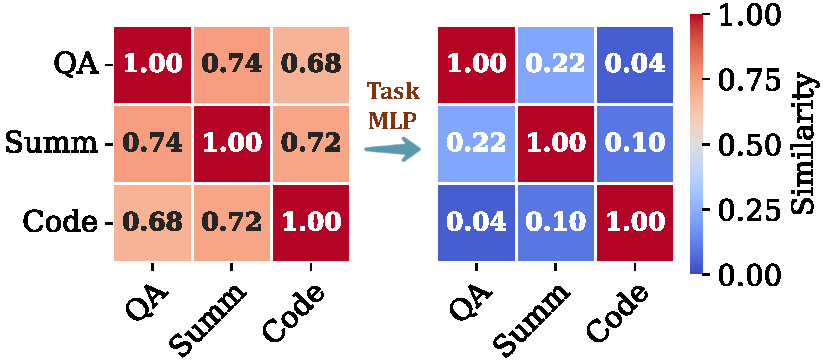
\includegraphics[width=\linewidth]{figures/task_heatmap.pdf}
    \vspace{-1.5em}
    \caption{任务表示相似度可视化。（左）Task MLP 之前，不同任务池化隐状态的两两余弦相似度较高；（右）经过 Task MLP 后，任务间相似度显著降低。}
  \label{fig:task_heatmap}
  
\end{figure}


\begin{table}[t]
    \centering
    \small
    \caption{不同 MLP 隐层维度的比较。}
    \label{tab:mlp_scale_ablation}
    \resizebox{\linewidth}{!}{
    \begin{tabular}{l|ccc|c}
        \toprule
        \textbf{隐层维度} & \textbf{LongBench} & \textbf{RULER} & \textbf{LongBench-V2} & \textbf{平均} \\
        \midrule
        $\mathbf{2\times d^{\prime}}$ & 48.07 & 60.67 & 26.92 & 45.22 \\
        % $\mathbf{3\times d^{\prime}}$ & 48.03 & - & 25.48 & - \\
        $\mathbf{4\times d^{\prime}}$（默认） & 48.08 & 61.81 & 27.88 & 45.92 \\
        $\mathbf{6\times d^{\prime}}$ & 48.07 & 62.08 & 26.20 & 45.45 \\
        $\mathbf{8\times d^{\prime}}$ & 48.47 & 65.27 & 25.48 & 46.40 \\
        \bottomrule
    \end{tabular}}
    \vspace{-0.5em}
\end{table}

\subsection{Attention Router 设计}
\label{abla:design_attn_router}

\paragraph{Task MLP 的作用}
我们分析 Attention Router 中 Task MLP 的作用。
具体地，我们取模型第一层的 Task MLP，计算任务隐状态（$x_K$）在通过 Task MLP 前后的两两余弦相似度。
余弦相似度越低，说明任务表示分离度越高，任务区分能力越强。
如图~\ref{fig:task_heatmap} 所示，我们在三类任务上比较后发现，经过 Task MLP 后任务间相似度明显下降。
这表明 Task MLP 能有效解耦任务特征，为后续 Router MLP 的路由决策提供更具判别性的表示。
更多细节及其他模型结果见附录~\ref{appendix:geometry_analysis}。


\begin{figure}[t]
  \centering
    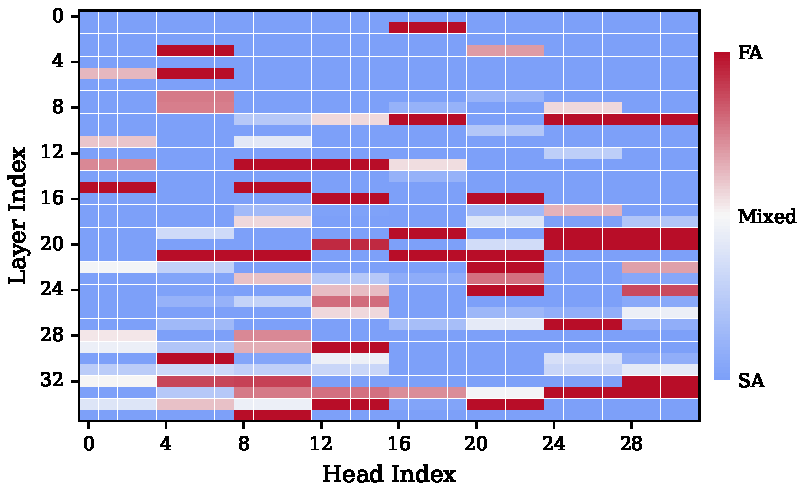
\includegraphics[width=\linewidth]{figures/qwen3-4b_per_task_head_robustness.pdf}
    \vspace{-1.5em}
    \caption{Qwen3-4B 中各头路由激活频率概览。红色表示在 LongBench-E 全部 6 个任务中始终被路由到 FA 的头（即检索头），蓝色表示始终被路由到 SA 的头。}
  \label{fig:robustness_heatmap}
\end{figure} 


\begin{figure}[t]
  \centering
    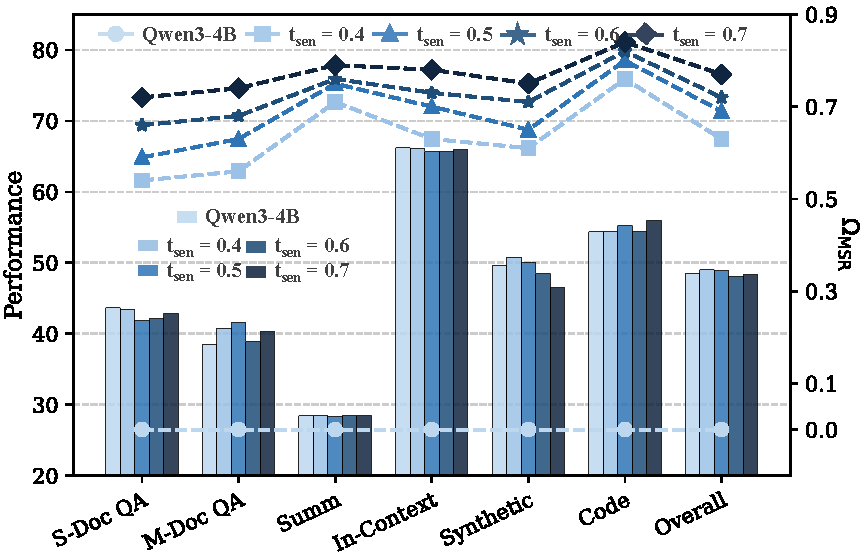
\includegraphics[width=\linewidth]{figures/diff_end_sparsity.pdf}
     \caption{不同训练目标稀疏度 $\boldsymbol{t}$ 设置下的性能与测试时 $\Omega_{\mathrm{MSR}}$ 对比。柱状图表示性能，折线图表示各任务的 $\Omega_{\mathrm{MSR}}$。}
  \label{fig:diff_end_sparsity}
  \vspace{-0.5em}
\end{figure}


\paragraph{MLP 中间隐层维度影响}
我们研究 Attention Router 中 Task-MLP 与 Router-MLP 的中间隐层维度对性能的影响。
具体测试范围为 $\times2 \sim\times8$，其中 $\times4$ 是主实验默认设置。
如表~\ref{tab:mlp_scale_ablation} 所示，所有设置在 3 个基准上的平均性能差异很小。
尽管 $\times8$ 取得最高总分，我们在主实验中仍采用 $\times4$，因为其在性能收益与额外参数开销之间更均衡。

\begin{figure*}[t]
\centering
  \begin{subfigure}[t]{0.33\textwidth}
    \centering
    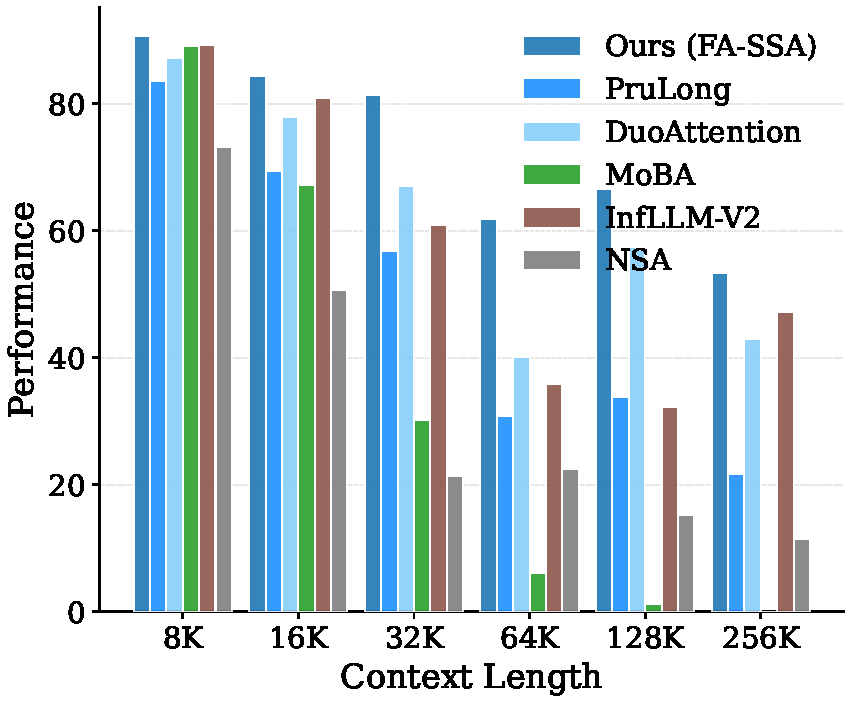
\includegraphics[width=\linewidth]{figures/side_by_side_streaming1.pdf}
    \caption{RULER 上的性能。}
    \label{fig:main_speedup_esr_1}
  \end{subfigure}
  \hfill
  \begin{subfigure}[t]{0.33\textwidth}
    \centering
    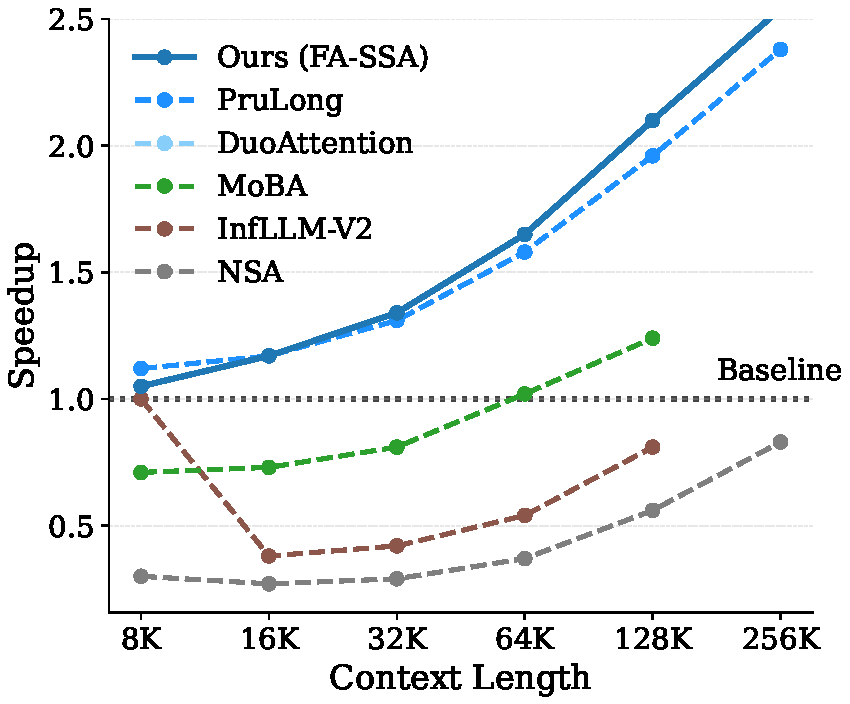
\includegraphics[width=\linewidth]{figures/side_by_side_streaming2.pdf}
    \caption{推理加速。}
    \label{fig:main_speedup_esr_2}
  \end{subfigure}
  \hfill
  \begin{subfigure}[t]{0.33\textwidth}
    \centering
    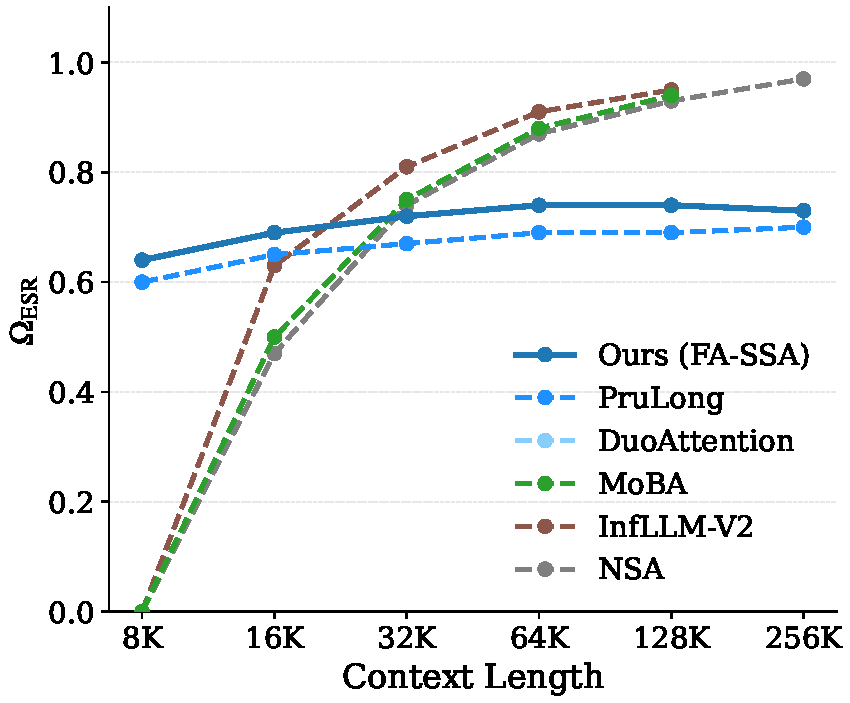
\includegraphics[width=\linewidth]{figures/side_by_side_streaming3.pdf}
    \caption{$\Omega_\mathrm{ESR}$ 统计。}
    \label{fig:main_speedup_esr_3}
  \end{subfigure}
\caption{不同方法在 RULER 上的性能与推理加速对比。以 Llama-3.1-8B-Instruct 为骨干，比较训练式方法（FA–SSA）与其他前沿稀疏注意力方法。我们报告 $\Omega_{\mathrm{ESR}}$，以公平比较不同方法在“实际被关注 token 比例”上的差异。}
\label{fig:main_speedup_esr}
\end{figure*}



\paragraph{注意力模式路由分析}
Attention Router 分配的注意力计算模式在头级别呈现稳定且一致的规律。
我们观察到，在 LLM 中部分头主要采用 FA，而另一些头则常被分配到 SA。
如图~\ref{fig:robustness_heatmap} 所示，我们分析了 LongBench-E 6 个子任务上各头的模式分布。
可以发现，一部分主要位于中高层的头在各任务中持续以 FA 模式激活。
这与 \citet{wu2024retrieval} 的发现一致，说明这些头具有检索头特性。
图中浅色高亮的部分头会在不同任务间切换，其余头则稳定路由到 SA。
更多结果见附录~\ref{appdix:head_analysis}。


\subsection{目标稀疏度 $\boldsymbol{t}$ 分配的影响}
\label{abla:sparsity_ratio_allocation}
我们研究目标稀疏度 $\boldsymbol{t}$（式~\ref{equ:training_ojective}）对模型性能的影响。
具体做法是固定稀疏鲁棒任务目标 $\boldsymbol{t}_\mathrm{rob}=1$，并将稀疏敏感任务目标 $\boldsymbol{t}_\mathrm{sen}$ 从 0.7 逐步降低到 0.4。
如图~\ref{fig:diff_end_sparsity} 所示，随着 $\boldsymbol{t}_\mathrm{sen}$ 降低，模型分配得到的 $\Omega_{\mathrm{MSR}}$ 在不同任务间的区分度略有提升。
但也可观察到，$\Omega_{\mathrm{MSR}}$ 并不会严格等于目标 $\boldsymbol{t}$。
原因在于我们采用的是\emph{任务相关且非紧约束}，不会强迫模型精确满足指定稀疏度。
完整训练曲线与解释见附录~\ref{appdix:loss_curve_monitoring_metrics}。
此外，当 $\boldsymbol{t}_\mathrm{sen}$ 过低（如 0.4）时，即分配更高比例 FA 计算，整体性能甚至可能超过骨干模型。
但从推理效率角度考虑，主实验采用 $\boldsymbol{t}_\mathrm{sen}=0.7$ 与 $\boldsymbol{t}_\mathrm{rob}=1.0$，在总体性能与推理效率之间取得更好平衡。

\subsection{整体性能与推理效率}
\label{abaa:esr_speedup}
我们在 RULER 多个上下文长度区间上比较不同方法的任务性能与推理效率。
实现细节见附录~\ref{appendix:baseline_train_setting}。
如图~\ref{fig:main_speedup_esr} 所示，我们的方法在所有对比方法中持续取得最佳性能。
同时，随着上下文长度增加，模型会动态分配更高 $\Omega_\mathrm{MSR}$，推理加速也随之提升。
相比之下，若干基线受限于架构设计。
例如 NSA 与 InfLLM-V2 对 KV 头数有严格整除约束（如 16 的倍数），与 Llama-3.1-8B 的配置并不匹配；此外 MoBA 与 InfLLM-V2 需要预留部分预算用于序列级特征预计算，在 256K 上下文下会出现 GPU 显存溢出。
最后，我们分析基于实际关注 token 数计算的 $\Omega_{\mathrm{ESR}}$。
结果表明，随序列长度增加，训练式混合模型的 $\Omega_{\mathrm{ESR}}$ 近似保持常数；而我们的方法能达到更低且更稳定的 $\Omega_{\mathrm{ESR}}$，并略优于可比基线（如 PruLong），体现了更好的有效稀疏可扩展性。
更多细节与对比见附录~\ref{appdix:length_extrapolation_and_sparsity_dynamics_analysis}。

\begin{table}[t]
    \centering
    \caption{将检索头替换为 XA 的结果。}
    \resizebox{\linewidth}{!}{
    \begin{tabular}{l|c c c | c}
    \toprule
    方法 & LongBench & RULER & LongBench-V2 & 平均 \\
    \midrule
    \rowcolor{blue!10}
    Qwen3-4B & 48.45 & 66.00 & 25.96 & 46.80 \\
    ~~+ XA-SSA & 48.14 & 63.70 & 25.96 & 45.93 \\
    \midrule
    \rowcolor{blue!25}
    Qwen3-8B & 52.16 & 75.74 & 31.97 & 53.26 \\
    ~~+ XA-SSA & 49.25 & 66.31 & 32.69 & 49.42 \\
    \midrule
    \rowcolor{cyan!20}
    Llama-3.1-8B & 53.28 & 83.47 & 32.69 & 56.48 \\
    ~~+ XA-SSA & 50.71 & 70.27 & 29.09 & 50.02 \\
    \bottomrule
    \end{tabular}}
    \label{abla:elastic_attn_scale}
\end{table}

\subsection{Elastic Attention 的可扩展性}
\label{abla:ela_attn_scale}
我们将检索头以 XA 实现，形成 XA–SSA 配置，使整个模型运行在全 SA 范式下，以评估 Elastic Attention 的可扩展性。
如表~\ref{abla:elastic_attn_scale} 所示，XA–SSA 仍能保持较强性能。
例如在 Qwen3-4B 上，3 个长上下文基准的平均性能差距仍可控制在 1 分以内。
尽管 8B 规模模型有一定性能下降，但这种权衡伴随显著推理加速，因为模型采用了完全稀疏注意力结构。







